\documentclass[tikz,border=10pt]{standalone}
\begin{document}
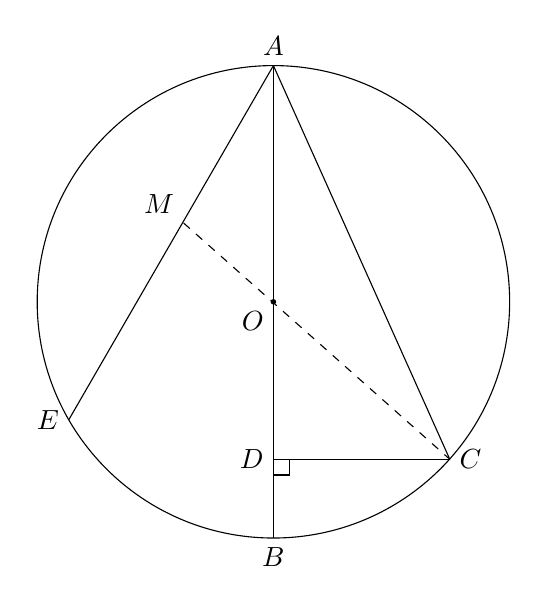
\begin{tikzpicture}
    \coordinate (O) at (0,0);
    \coordinate (A) at (0,3);
    \coordinate (B) at (0,-3);
    \coordinate (C) at (2.24, -2);
    \coordinate (D) at (0, -2);
    \coordinate (E) at (-2.6, -1.5);
    \coordinate (M) at (-1.14, 1.0);
    
    \draw (O) circle (3);
    \draw (A) -- (B);
    \draw (A) -- (C);
    \draw (A) -- (E);
    \draw (C) -- (D);
    \draw[dashed] (M) -- (C);
    
    % Right angle mark at D
    \draw (D) ++(0.2, 0) -- ++(0, -0.2) -- ++(-0.2, 0);
    
    \fill (O) circle (1pt);
    
    \node[above] at (A) {$A$};
    \node[below] at (B) {$B$};
    \node[right] at (C) {$C$};
    \node[left] at (D) {$D$};
    \node[left] at (E) {$E$};
    \node[above left] at (M) {$M$};
    \node[below left] at (O) {$O$};
\end{tikzpicture}
\end{document}
